\lhead{\emph{\ChapterThree{}}}
\label{classification-conclusions}
El primer acercamiento de clasificación se realizó utilizando los metadatos disponibles para cada uno de los TFGs, concretamente el título y el abstracto. Se utilizó el campo de "tema" para determinar la clasificación que se le había dado a cada TFG en el RIULL.
%

Se realizó una batería de pruebas, variando el número de palabras comunes a considerar. Se empezó utilizando las 100 palabras más comunes, aumentando esto en incrementos de 100 hasta llegar a un clasificador que considera las 2000 palabras más comunes entre los textos a clasificar.

\begin{center}
\begin{figure}[!ht]
  \label{fig:metadata_view}
  \centering
    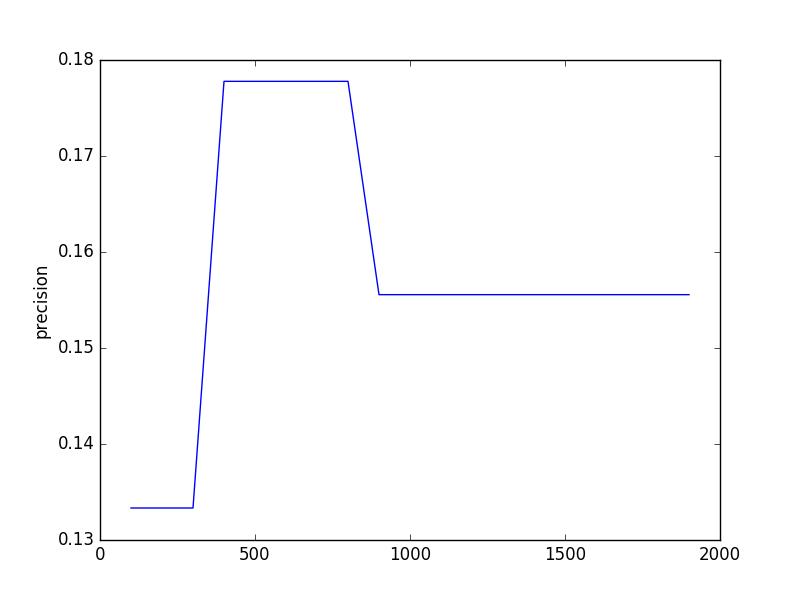
\includegraphics[width=0.8\textwidth]{Images/figure_1}
  \caption{Precisión de la clasificación Naive Bayes usando metadatos de los TFG de Ing. Informática.}
\end{figure}
\end{center}

Como vemos, la precisión del clasificador oscila entre 0.13 y 0.18, lo que indica que el clasificador acierta entre el 13\% y 18\% de las veces. Estos resultados son bastante pobres, y esto se debe a la poca información que proporcionan los metadatos existentes sobre los textos.
%
La falta de información se debe a tres factores: en primer lugar, los títulos no suelen sobrepasar las 20 palabras, lo que hace difícil la clasificación por conteo de palabras comunes. 
%
El segundo problema es que en muchos casos, la descripción o abstracto del TFG no se encuentra como metadato del TFG en la RIULL, debido a ser un campo opcional.
%
Finalmente, se tiene un número elevado de clases, muchas de ellas conteniendo a un único TFG, lo que reduce las posibilidades de caracterizar una clase y aumenta las probabilidades de cometer una asignación errónea.

Por otra parte, podemos observar cómo decrementa la precisión del clasificador a partir de un número de palabras dado. Podemos inducir de esto que existe un límite de palabras a considerar óptimo, tras el cual se consideran demasiadas características de los elementos como para dar una respuesta fiable.